% !TEX root = ../thesis.tex
\section{Conclusion}\label{sec:conclusion}

In this thesis, we have addressed the research question on how to connect different mathematical knowledge systems
in a generic, efficient and scalable manner to enable transparent, semantics-aware, distributed computation. 

To do this, we decided to make use of the Math-In-The-Middle paradigm. 
Using Virtual Theories, QMT and SCSCP we have created a solution that indeed provides a solution to this question. 
To achieve this we have had to address all three initial aspects. 

\begin{description}
  \item[A generic mechanism to manage and sync knowledge stored in MKS]\quad\\
    Using \lmfdb\ as an example, we have seen how to build a virtual theory layer acting as such a mechanism.  
    Our core contribution here is the choice of using Codecs to ensure separation of semantic and realized types. 
    This choice has turned out exactly right -- enabling our mechanism to easily integrate with different systems while at the same time not being ad-hoc. 
    This makes it different and better than existing approaches. 
    
  \item[A System-Independent Query Language]\quad\\
    We have furthermore built on top of the existing QMT language of the MMT system. 
    Instead of choosing to use a query language that relies on a specific data structure we can now see that we made the right choice here. 
    
    QMT was designed from the ground up to enable formulation of representation-independent queries. 
    Even though it required a refactoring and some extensions to properly deal with distributed computations, we have seen that this choice fits in well with the mechanism of codecs and almost naturally extends the knowledge representational aspects of the MiTM approach to computational ones. 
  
  \item[A Lower-Level Communication Layer] \quad\\
    For this layer, we choose to use the SCSCP protocol. 
    Along with the other two layers, and especially inside this one, we can see how it was a good choice to build on a system-independent framework. 
    The representation of objects using OpenMath or \omdocmmt\ terms enabled systems to easily expose their computational functionality. 
    This reaffirms again that communication between different specialist systems is possible without having to rely on an industry standard of having to rely on ad-hoc solutions -- a generic pattern like the one here is possible. 
\end{description}

To reflect on our contribution further, we take a final look at Jane's initial example of cross-system communication. 

\subsection{Revisiting the Use-Case For Cross-System Communication}\label{sec:conclusion:example}

With all the pieces in place, we can now see how our architectural choices help Jane express her computational problem in QMT. 

\begin{example}\label{example:cross}
  Jane's example expressed as a QMT Query. 
  \begin{lstlisting}[language=qmt]
  use "gap" for (
    use "lmfdb" for {*
      x in (
        related to ( literal `lmfdb:db/transitivegroups?group ) by (object declares)
      ) | holds x (
        x commutative x *=* true
      )
    *} 
  ) map x => cyclic x)
  \end{lstlisting}
\end{example}

% !TEX root = ../thesis.tex
\begin{figure}[h]
  \begin{center}
    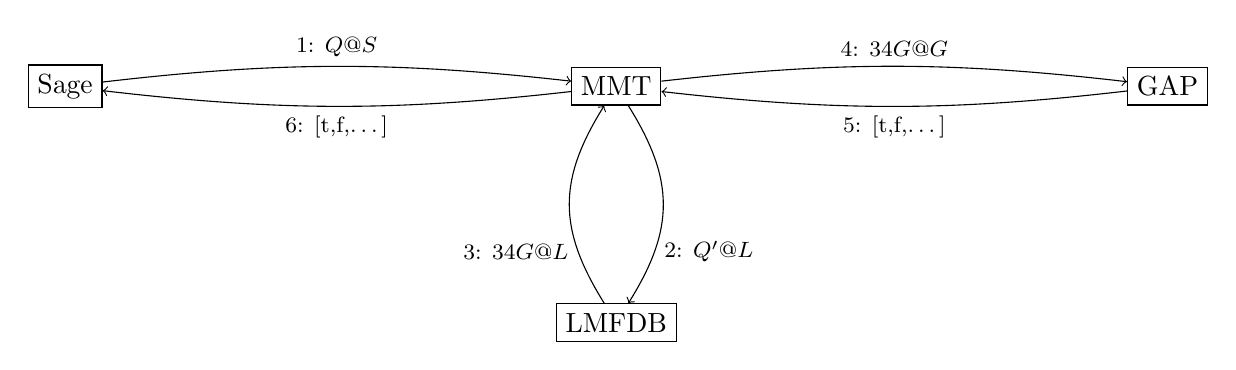
\begin{tikzpicture}[xscale=7,yscale=3]\normalsize
      \node[draw] (s) at (0,0) {Sage};
      \node[draw] (m) at (1,0) {MMT};
      \node[draw] (g) at (2,0) {GAP};
      \node[draw] (l) at (1,-1) {LMFDB};
      \draw[->] (s) to[bend left=15] node[above] {\footnotesize 1: $Q@S$} (m);
      \draw[->] (m) to[bend left=15] node[right,near end] {\footnotesize 2: $Q'@L$} (l);
      \draw[<-] (m) to[bend right=15] node[left,near end] {\footnotesize 3: $34G@L$} (l);
      \draw[->] (m) to[bend left=15] node[above] {\footnotesize 4: $34G@G$} (g);
      \draw[<-] (m) to[bend right=15] node[below] {\footnotesize 5: [t,f,\ldots]} (g);
      \draw[<-] (s) to[bend right=15] node[below] {\footnotesize 6: [t,f,\ldots]} (m);
    \end{tikzpicture}
  \end{center}

  \caption[A MiTM use-case]{
    Elaborated technical details for Cross-System-Communication Use-Case. 
    Compare with Figure~\ref{fig:mitmcaseintro}. 
  }
  \label{fig:mitmcase}
\end{figure}
We can now also have another look at Figure~\ref{fig:mitmcaseintro}. 
In Figure~\ref{fig:mitmcase} the steps of this process are annotated with more technical details. 
\begin{enumerate}
  \item Jane formulates a QMT Query which expresses this hypothesis and sends it to \mmt. 
  This is the one shown above and consists of two parts. 
  The first part uses \lmfdb\ to retrieve all abelian (commutative) groups from \lmfdb. 
  This sub-query corresponds to Example~\ref{example:lmfdblong} and is in lines 2-8. 
  The second part uses GAP to check if a group is indeed cyclic. 
  Here, another \identifier{I()} query is used (line 1) to check if each of the results is indeed cyclic by using \identifier{map}. 
  
  \item \mmt\ identifies the inner \lmfdb\ query, translates and sends it to the \lmfdb API. 
  
  \item \mmt\ receives a list of $34$ results from \lmfdb\ and translates these back into Math-In-The-Middle terms. 
  
  \item \mmt\ then translates these intermediate results into objects that GAP can understand. 
  Next it translates the remainder of the query, and sends it to GAP along with the intermediate results using the SCSCP protocol. 
  
  \item GAP responds to the query and sends back a list of $34$ boolean (OpenMath) objects.
  This lists contains both \inlinecode{true} and \inlinecode{false}, because it turns out that the original hypothesis is false. 
  
  \item Finally, \mmt\ translates this set of results into a Sage objects which are then delivered back to Jane. 
\end{enumerate}

Most of these steps are hidden from Jane -- she only sends a single QMT Query. 
This makes this example truly a transparent, distributed cross-system communication. 

As we have seen the approach maintains object semantics across systems -- this is illustrated by Jane never seeing a $0$ or a $1$ which is stored inside of \lmfdb. 
Furthermore, she never knows that the abelian is stored in \lmfdb\ as the \identifier{ab} property -- no insight into \lmfdb\ is required. 

\subsection{Outlook}\label{sec:conclusion:outlook}

Currently, steps 1 - 5 in are implemented inside of \mmt\ and are fully functional. 
This once again shows that the MiTM approach is suitable of facilitating cross-system communication and was a valid choice. 
Furthermore, the approaches above are indeed feasible and improve on existing systems. 

However, work in this area is far from complete. 
Apart from extending the approach to include more systems and testing it in more settings, 
there are a several improvements that can be made. 

Consider for example QMT. 
Currently, sub-queries need manual annotation to mark them as being used with external systems. 
During this thesis it has been speculated that an automatic approach intercepting each intermediate result would be to computationally expensive. 
In a future extension of the query language, one might instead consider analyzing the structure of each query and automatically annotating parts of the query to be evaluated with different systems. 

Furthermore, as stated above, step 6 of the example has not yet been implemented. 
This means making QMT available to the Sage system.
Thus we need to implement one of two approaches, either make a Sage specific API, or exposing the QMT interface via SCSCP and building a client inside of Sage. 
The latter of these options seems appealing, and has been hinted on during this thesis. 
However, this approach requires more thought than might initially seem necessary. 

It is straightforward to send queries from Sage, however it is not as easy to receive the results. 
As stated above, these need to be translated into something that Sage specific. 
Hence, when posing the Query, \mmt\ needs to be made aware that the Query is coming from Sage. 
To implement this in a generic fashion that can eventually be extended to systems beyond the ones mentioned here, one could either add a separate case to the query language, or build this into an argument to be passed only via SCSCP. 
  
\subsection{Acknowledgements}\label{sec:conclusion:outlook:acknowledgements}

The author acknowledges that the work for this project has been financially supported by the OpenDreamKit Horizon 2020 European Research Infrastructures project (\#676541). 
Furthermore, the author expresses his thanks to John Cremona for his help on understanding the structure of objects inside of \lmfdb\ as well as all members of the KWARC group, and in particular Michael Kohlhase, for their input and help during the design and implementation phases of the work described here. 